\documentclass[aspectratio=169,xcolor=dvipsnames,pdf]{beamer}
% \usetheme{SimpleDarkBlue}
\usetheme[black]{NXYZ} % Black theme

\setbeamerfont*{frametitle}{size=\Large, series=\bfseries, parent=structure}

\AtBeginSection[]{
    \begin{frame}
    \vfill
    \centering
    \begin{beamercolorbox}[sep=8pt,center,shadow=true,rounded=true]{section page}
        \usebeamerfont{title}%
        \textit{\thesection~}%
                {\color{black} \insertsectionhead}\par%
    \end{beamercolorbox}
    \vfill
    \end{frame}
}

% German language
\usepackage[ngerman]{babel}
\usepackage[utf8]{inputenc}
\usepackage[T1]{fontenc}

% add graphics
\usepackage{graphicx}
\usepackage{dblfloatfix}

% lets tables span over page
\usepackage{tabularx}

% code block	
\usepackage{listings}
\usepackage{xcolor}

\definecolor{backcolour}{RGB}{245, 245, 245}

\lstdefinestyle{codestyle}{
	backgroundcolor=\color{backcolour},
    commentstyle=\color{gray},
    numberstyle=\ttfamily\scriptsize,
    basicstyle=\ttfamily\footnotesize,
    breakatwhitespace=false,         
    breaklines=true,                 
    captionpos=b,                    
    keepspaces=true,                 
    % numbers=left,                    
    numbersep=5pt,                  
    showspaces=false,                
    showstringspaces=false,
    showtabs=false,                  
    tabsize=2,
    % xleftmargin=0.15in
}

\lstset{style=codestyle}

\lstdefinestyle{tinycodestyle}{
	backgroundcolor=\color{backcolour},
    commentstyle=\color{gray},
    numberstyle=\ttfamily\tiny,
    basicstyle=\ttfamily\tiny,
    breakatwhitespace=false,         
    breaklines=true,                 
    captionpos=b,                    
    keepspaces=true,
    % numbers=left,                    
    numbersep=5pt,                  
    showspaces=false,                
    showstringspaces=false,
    showtabs=false,                  
    tabsize=2,
    % xleftmargin=0.15in
}

\lstset{style=tinycodestyle}

% for hyperlinks
\usepackage{hyperref}

% for titlepage
\title{Generierung von Schachkommentaren}
\subtitle{mittels maschinellem Lernen}
\author{Max Semdner}
\institute{Frankfurt University of Applied Sciences}
\date{31. Januar 2023}

\begin{document}

% Titlepage frame
\begin{frame}
\titlepage
\end{frame}

% Table of Contents
\begin{frame}{Table of Contents}
\tableofcontents
\end{frame}

\section{Einführung}

Willkommen zu meiner Presentation mit dem Titel ``Generierung von Schachkommentaren mittels maschinellem Lernen''.\\

Zu Beginn werde ich Ihnen einen Überblick darüber geben, wie die Themen Schach und künstliche Intelligenz zusammenhängen, damit die Notwendigkeit meiner Forschungsfrage deutlich wird. Dann werde ich kurz den Aufbau zur Lösung der Forschungsfrage vorstellen.\\

In den Abschnitten 2 und 3 wird der Aufbau näher erläutert, und Abschnitt 4 schließt die Präsentation mit einem Fazit ab.

\section{Überblick}

Schach gehört zu einem der am längsten erforschten Themen der Künstlichen Intelligenz. Das liegt vor allem daran, dass Pioniere der KI wie Alan Turing Schachspieler waren und das Schachspiel als ideales Modell für maschinelles Lernen betrachteten.\\

Damals wie heute wurde hauptsächlich auf dem Gebiet der Schachengines geforscht. Das sind Schachprogramme. Das Ziel der Forschung ist es, die Spielstärke zu optimieren. Heute liegt die Spielstärke der Engiens weit über der der besten Profispieler.\\

Ein Problem ist, dass dieses hohe Spielniveau zu einer Intransparenz von Zügen bzw. Zugfolgen führt. Das bedeutet, dass man professionelle Spieler oder Kommentatoren braucht, um die Ideen hinter den Zügen des Computers zu verstehen, und selbst deren Analysen sind nicht immer korrekt.\\

Meine Forschungsfrage "Wie kann maschinelles Lernen genutzt werden, um Kommentare zu Schachpartien zu generieren?" versucht, dieses Problem der Intransparenz von Zügen zu lösen, indem versucht wird, menschliche Kommentatoren durch virtuelle zu ersetzen.

\newpage

Um die Forschungsfrage zu lösen, teilen wir sie in zwei Teile. Zum einen die Informationsbeschaffung und die Kommentarerstellung. Die Informationsbeschaffung befasst damit \textit{woher} wir Informationen bekommen die zum übersetzen nötig ist. Die Kommentargenerierung nimmt diese Informationen und beschäftigt dann damit \textit{wie} und \textit{was} für Kommentare erzeugt werden sollen.\\

Für den ersten Teil wird eine bereits erwähnte Schach Engine verwendet, für den zweiten Teil das sogenannte Encoder-Decoder-Modell.\\



\section{Schachkommentator}

\subsection{Encoder-Decoder Modell}

% ================================================================================ %
\begin{frame}{Encoder-Decoder Modell}
\begin{itemize}
	\item Schachkommentator nimmt Informationen und übersetzt sie in Kommentare
	\item Bereich: Sequence-to-sequence processing
	\begin{itemize}
		\item Abbildung einer Eingabe auf eine Ausgabe
	\end{itemize}
	\item Architektur: Encoder-Decoder Modell
	\begin{itemize}
		\item Basierend auf bidirektionalen Long Short-Term Memory (LSTM)
	\end{itemize}
\end{itemize}
\end{frame}




\begin{frame}{Encoder-Decoder Modell}
\begin{itemize}
	\item LSTMs sind eine spezielle Art von Rekurrenten Neuronalen Netzwerken
	\item RNNs sind Neuronale Netzwerke zur Verarbeitung von Datenfolgen
	\begin{itemize}
		\item Outputs werden mit neuen Inputs an das Netzwerk gegeben
		\item Zustand des Netzes repräsentiert Neuronen zu einem bestimmten Zeitpunkt
		\item Netzwerk kann sich an laufende Muster erinnern und auf diese reagieren
	\end{itemize}
	\item Bidirektionale RNNs (Bi-RNN) sind eine Erweiterung von RNNs
	\begin{itemize}
		\item Berücksichtigen sowohl die vorherigen als auch die nachfolgenden Eingabedaten
	\end{itemize}
	\item LSTMs sind spezielle Neuronen
	\begin{itemize}
		\item Bei langen Sequenzen werden die Informationen aus der Vergangenheit nicht korrekt berücksichtigt
		\item LSTMs lösen das Problem
	\end{itemize}
\end{itemize}
\end{frame}




\begin{frame}{Encoder-Decoder Modell}
\begin{itemize}
	\item Encoder-Decoder Modell benutzt Bi-LSTMs
	\begin{itemize}
		\item in der maschinellen Übersetzung verwendet
	\end{itemize}
	\item Besteht aus zwei Teilen: Encoder, Decoder
	\begin{itemize}
		\item Encoder erhält Eingabe von Engine und wandelt diese in andere Darstellung um
		\item Decoder verwendet diese Darstellung und erstellt entsprechende Kommentare
	\end{itemize}
	\item Aufmerksamkeitsmechanismus wird verwendet, um auf wichtige Teile der Sequenz zu konzentrieren
\end{itemize}
\end{frame}




\begin{frame}{Encoder-Decoder Modell}
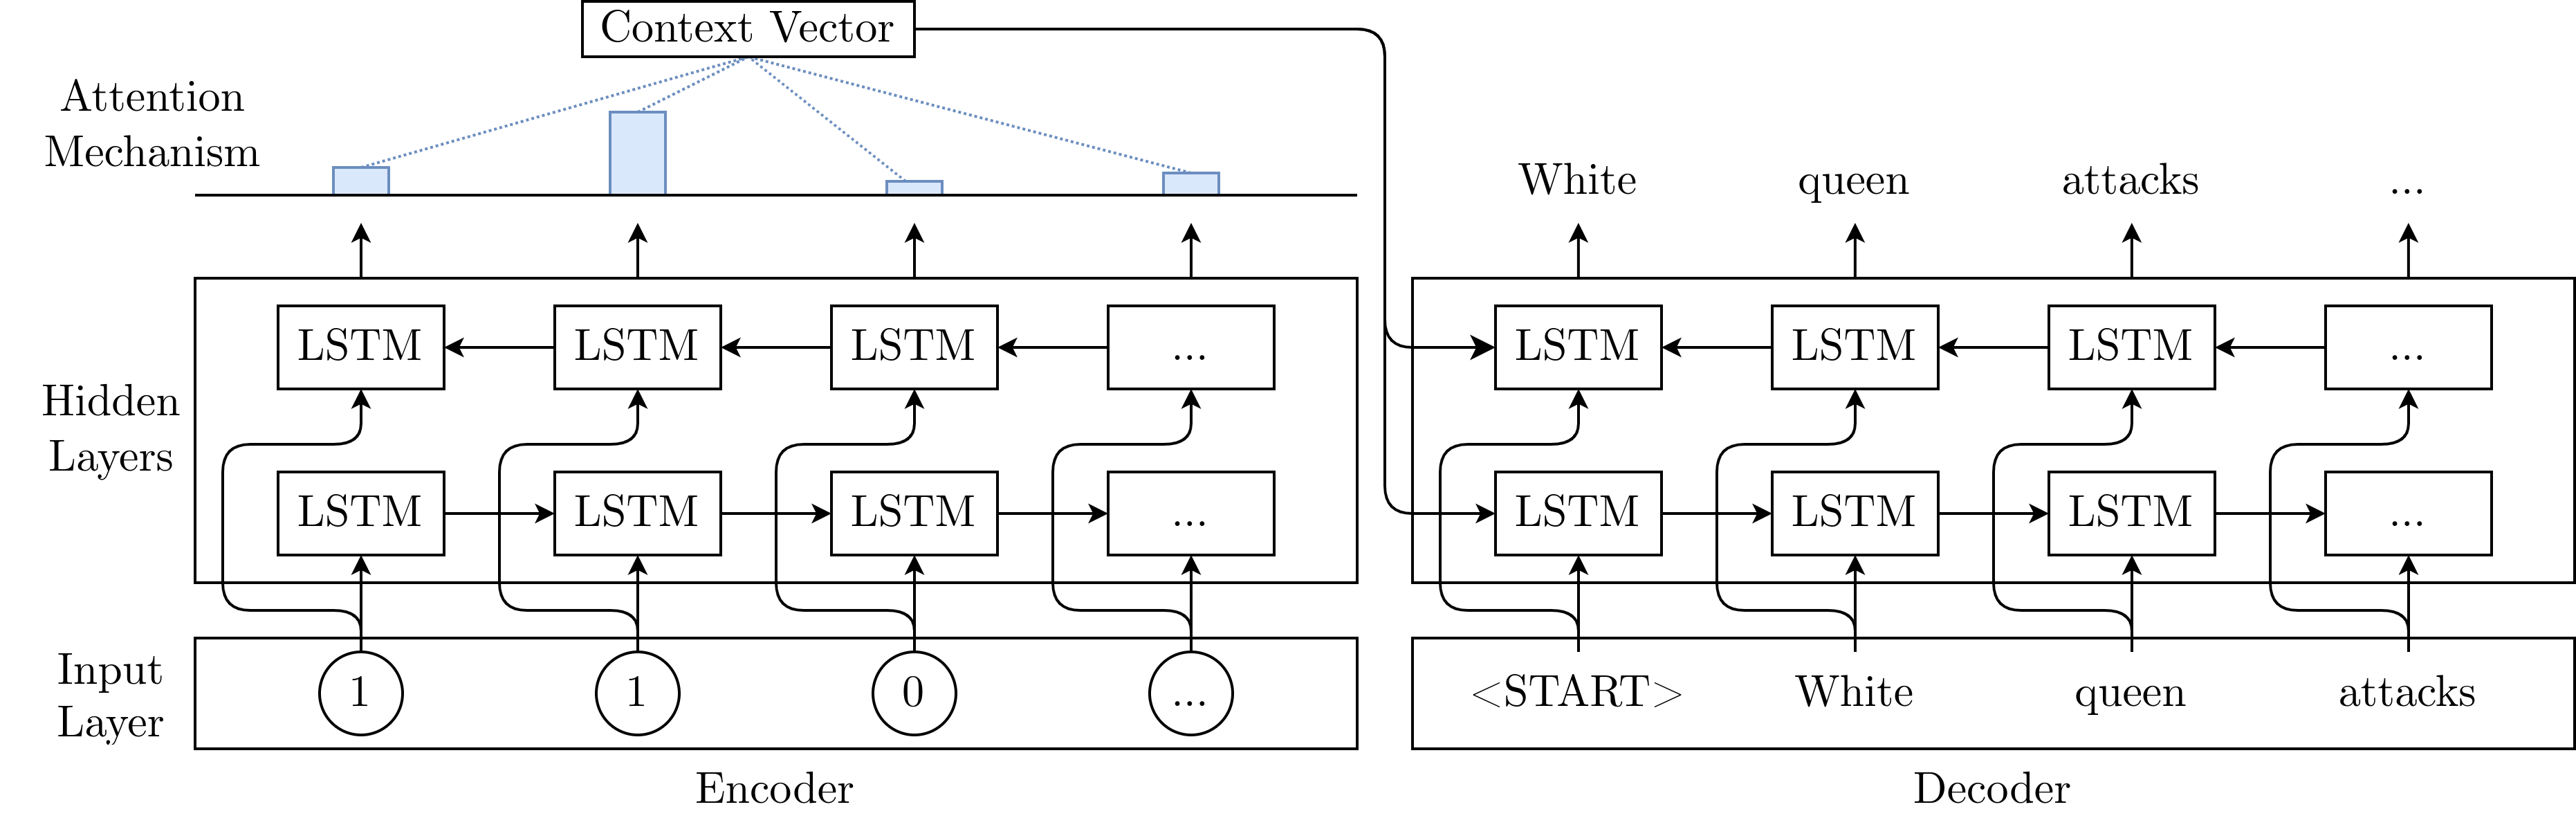
\includegraphics[width=1\textwidth]{graphics/commentator_example/general_approach.png}
\end{frame}
% ================================================================================ %

\subsection{Generationsmodelle}

% ================================================================================ %
\begin{frame}{Generationsmodelle}
\begin{itemize}
	\item Es muss definiert werden, welche Kategorien von Kommentaren generiert werden sollen
	\begin{itemize}
		\item Beschreibung
		\item Qualität
		\item Vergleich
		\item Planung
		\item Kontext
	\end{itemize}
\end{itemize}
\begin{figure}
\centering
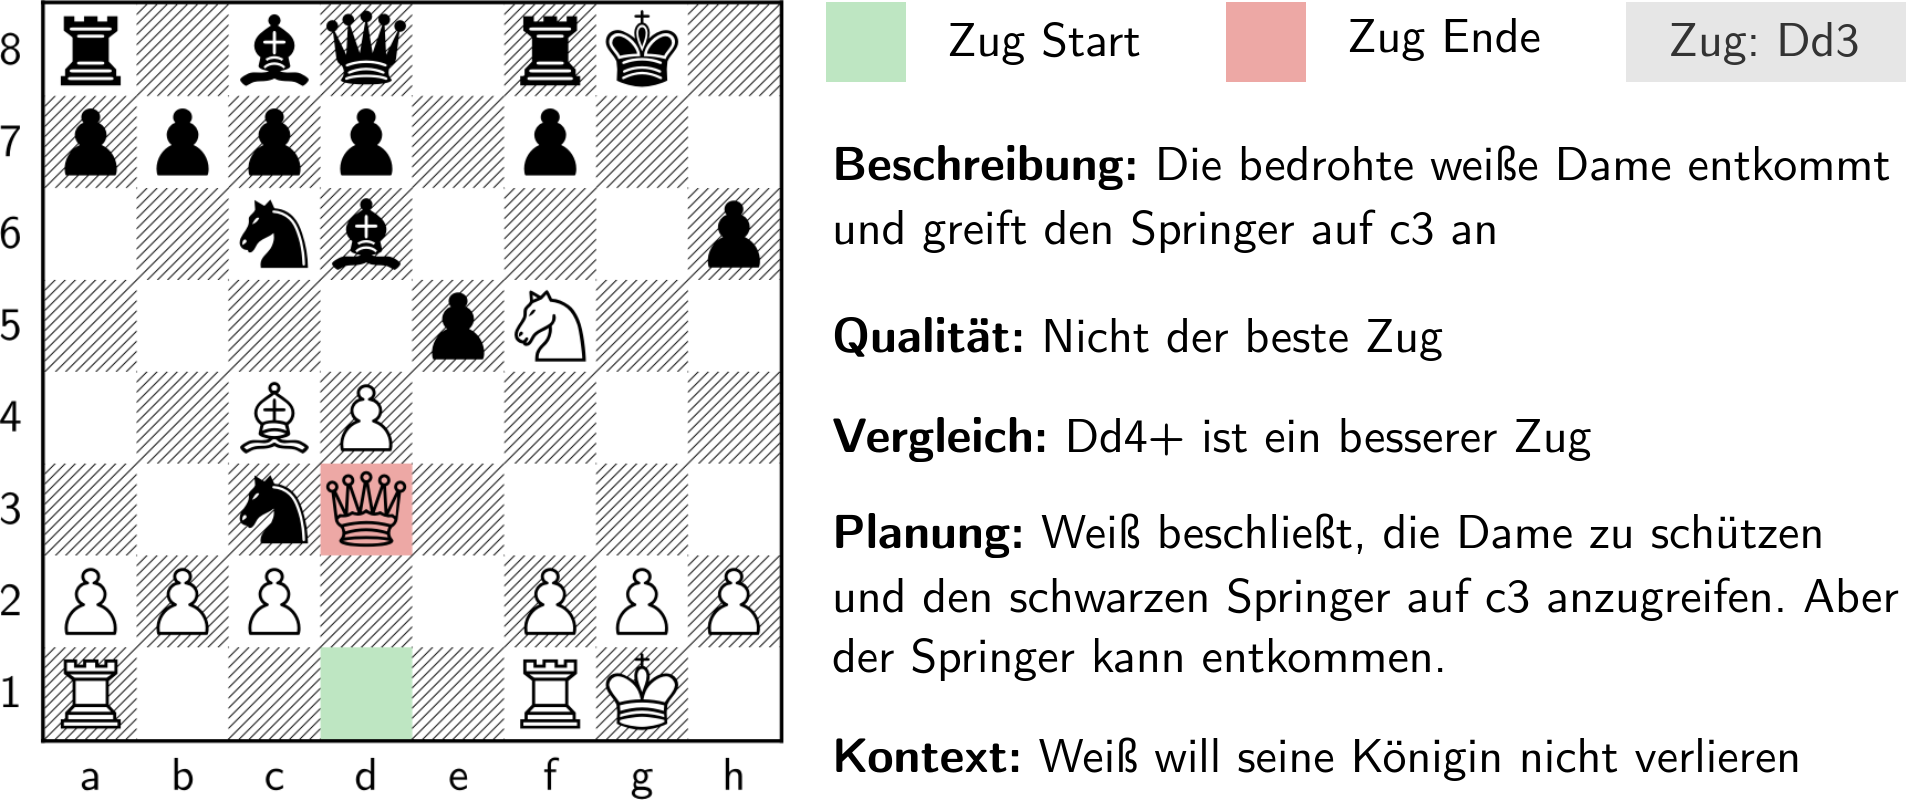
\includegraphics[width=0.55\textwidth]{graphics/commentator_example/commentator.png}
\end{figure}
\end{frame}




\begin{frame}{Generationsmodelle}
\begin{itemize}
	\item Einzelner Kommentator nicht aus
	\item Für jede Kategorie ein Kommentator in Form von Encoder-Decoder Modell (sog. Generationsmodelle)
	\item Generationsmodelle unterscheiden sich im Training
	\begin{itemize}
		\item Unterschiedliche Merkmale und Anzahl an Zügen werden berücksichtigt
	\end{itemize}
\end{itemize}
\end{frame}




\begin{frame}{Generationsmodelle}
\begin{itemize}[<+->]
	\item Zug $m$, Position $b$ 
	\item \textbf{Beschreibung:} $f_{Decoder}(f_{SME}(b_0,m_0)) \rightarrow C_{Beschreibung}$
	\item \textbf{Qualität:} $f_{Decoder}(f_{Encoder}(b_0,b_1,v_1-v_0)) \rightarrow C_{Qualitaet}$
	\item \textbf{Vergleich:} $f_{Decoder}(f_{MME}(b_1,m_0,b_2,m_1)) \rightarrow C_{Vergleich}$
	\item \textbf{Planung:} $f_{\text{Decoder}}(f_{\text{MME}}((b_2,m_1),(b_3,m_2),(b_4,m_3),...)) \rightarrow C_{\text{Planung}}$
	\item \textbf{Kontext:} $f_{\text{Decoder}}(f_{\text{MME}}((b_1,m_0),(b_2,m_1),(b_3,m_2),(b_4,m_3),...)) \rightarrow C_{\text{Kontext}}$
\end{itemize}
\end{frame}
% ================================================================================ %

\section{Schachkommentator}

Jetzt werden ich den Teil besprechen, der für die Erzeugung von Kommentaren verantwortlich ist.

\subsection{Encoder-Decoder Modell}

Die Erzeugung von Kommentaren fällt in den Bereich der Sequenz-zu-Sequenz-Verarbeitung, was bedeutet, dass ein Input (hier entsprechende Informationen) auf einem Output (d.h. menschliche Sprachen) dargestellt wird. Länge von Input und Output können sich dabei unterscheiden.\\

Eine Architektur die dies ermöglicht ist das Encoder-Decoder Modell.\\

Das Modell basiert auf einer speziellen neuronalen Netzwerkarchitektur, der so genannten bidirektionalen Long-Short Term Memory-Architektur. Bevor ich das Encoder-Decoder Modell erkläre, gehe ich kurz auf diese Architektur ein.

\newpage

LSTMs sind eine Erweiterung von Rekurrenten Neuronalen Netzwerken\\

RNNs sind neuronale Netze, die zur Verarbeitung von Sequenzen geschaffen wurden. Dabei werden die generierten Outputs wieder mit neuem Input in das Netzwerk geben. Der Zustand des Netzes repräsentiert die Neuronen also zu einen bestimmten Zeitpunkt. Durch das zurückführen des Outputs kann sich das Netzwerk an laufende Muster erinnern und entsprechend darauf reagieren.\\

Bidirektionale RNNs sind eine Erweiterung der RNNs. Eingaben werden nicht nur in positiver Zeitrichtung, sondern auch in negativer Zeitrichtung berücksichtigt. D.h. es werden sowohl die vorherigen als auch die nachfolgenden Eingabedaten einbezogen.\\

Ein Problem, das bei RNNs auftritt, ist, dass sie sich zwar länger laufende Muster merken können, dieses Gedächtnis aber Probleme mit langen Sequenzen hat. Dieses Problem wird als das Problem des verschwindenden Gradienten bezeichnet. LSTMs sind spezielle Neuronen, die dieses Problem lösen. Sie verfügen über ein Kurzzeitgedächtnis und ein Langzeitgedächtnis, so dass die Muster auch bei langen Sequenzen genau gespeichert werden.\\

Bidirektionale LSTMs sind also bidirektionale RNNs, die die Long-Short Term Memory Neuronen verwenden.

\newpage

Das Encoder-Decoder Modell besteht aus zwei Teilen dem Encoder, Decoder. Bei beiden handelt es sich um Bidirektionale LSTMs.\\

Der Encoder empfängt als Input die Informationen von der Schach-Engine und wandelt sie in eine andere Darstellung um. Diese Darstellung ist eine Zusammenfassung der Informationen. Die Zusammenfassung wurde mit Hilfe eines Aufmerksamkeitsmechanismus erstellt.\\

Der Decoder verwendet dann diese Darstellung und erstellt entsprechende Kommentare.

\newpage

Hier habe ich eine Abbildung so eines Encoder-Decoder Modells mitgebracht.\\

Eine dieser Blöcke stellt das Netzwerk zu einem bestimmten Zeitpunkt dar, von links nach rechts werden zeitlich aufsteigend die entsprechenden Sequenz eingegeben.\\

Die Hidden Layers verarbeiten die Sequenz und durch einen Aufmerksamkeitsmechanismus werden bestimmte Teile der Eingabe zusammengefasst und zu einem Endzustand kombiniert. Dieser Zustand wird auch als Kontextvektor bezeichnet.\\

Der Kontextvektor wird dann zur Initialisierung der Neuronen des Decoders verwendet. Um Kommentare zu erzeugen, wird ein Startzeichen als Eingabe eingegeben, und die Ausgabe stellt den erzeugten Kommentar dar. Die Ausgabe wird als neue Eingabe in den Decoder gegeben. Dies geschieht so lange, bis ein Endzeichen erreicht wird, das das Ende des Kommentars signalisiert.

\newpage

\subsection{Generationsmodelle}

Um zu wissen zu was genau man Kommentare generieren soll, wurde 5 Kategorien festgelegt.\\

Das Problem ist, dass es für Encoder-Decoder Modell nicht ausreicht. Deshalb wird für jede dieser Kategorien ein Encoder-Decoder Modell verwendet welche sich im Training unterscheiden. Die Kategorien, werden deshalb auch Generationsmodelle genannt.\\

Das Training der Generationsmodelle unterscheiden sich in der Merkmalen die diese zum Trainieren bekommen sowie die Anzahl der Züge.

Encoder die mehrere Züge bekommen werden dabei als Multi-Move-Encoder bezeichnet, Encoder die nur einen Zug bekommen als Single-Move-Encoder.\\

Welche Merkmale die Modelle erhalten, lässt sich als Funktion zusammenfassen. Ein Zug wird dabei mit $m$ für move abgekürzt und eine Position mit $b$ für board.\\

Nun da man weiß was für Merkmale man zum trainieren brauch, wurden Datensätze zum Trainieren, erstellt, welche basierend auf Kommentaren aus den fünf Kategorien aus einem Schachforum stammen.

\end{document}

